% !TeX root = ../main.tex

\chapter{LXeTPC与HPGe探测器的工作原理}

了解探测器的结构和信号产生过程对于信号测量和本底估计必不可少,
本章将以暗物质探测实验中的LXeTPC和HPGe探测器应用为基础,介绍两类探测器的工作原理,
并设计一种能够在地面反应堆附近运行的LXeTPC探测器及屏蔽体结构。

\section{LXeTPC的基本工作过程}

\begin{figure}
    \centering
    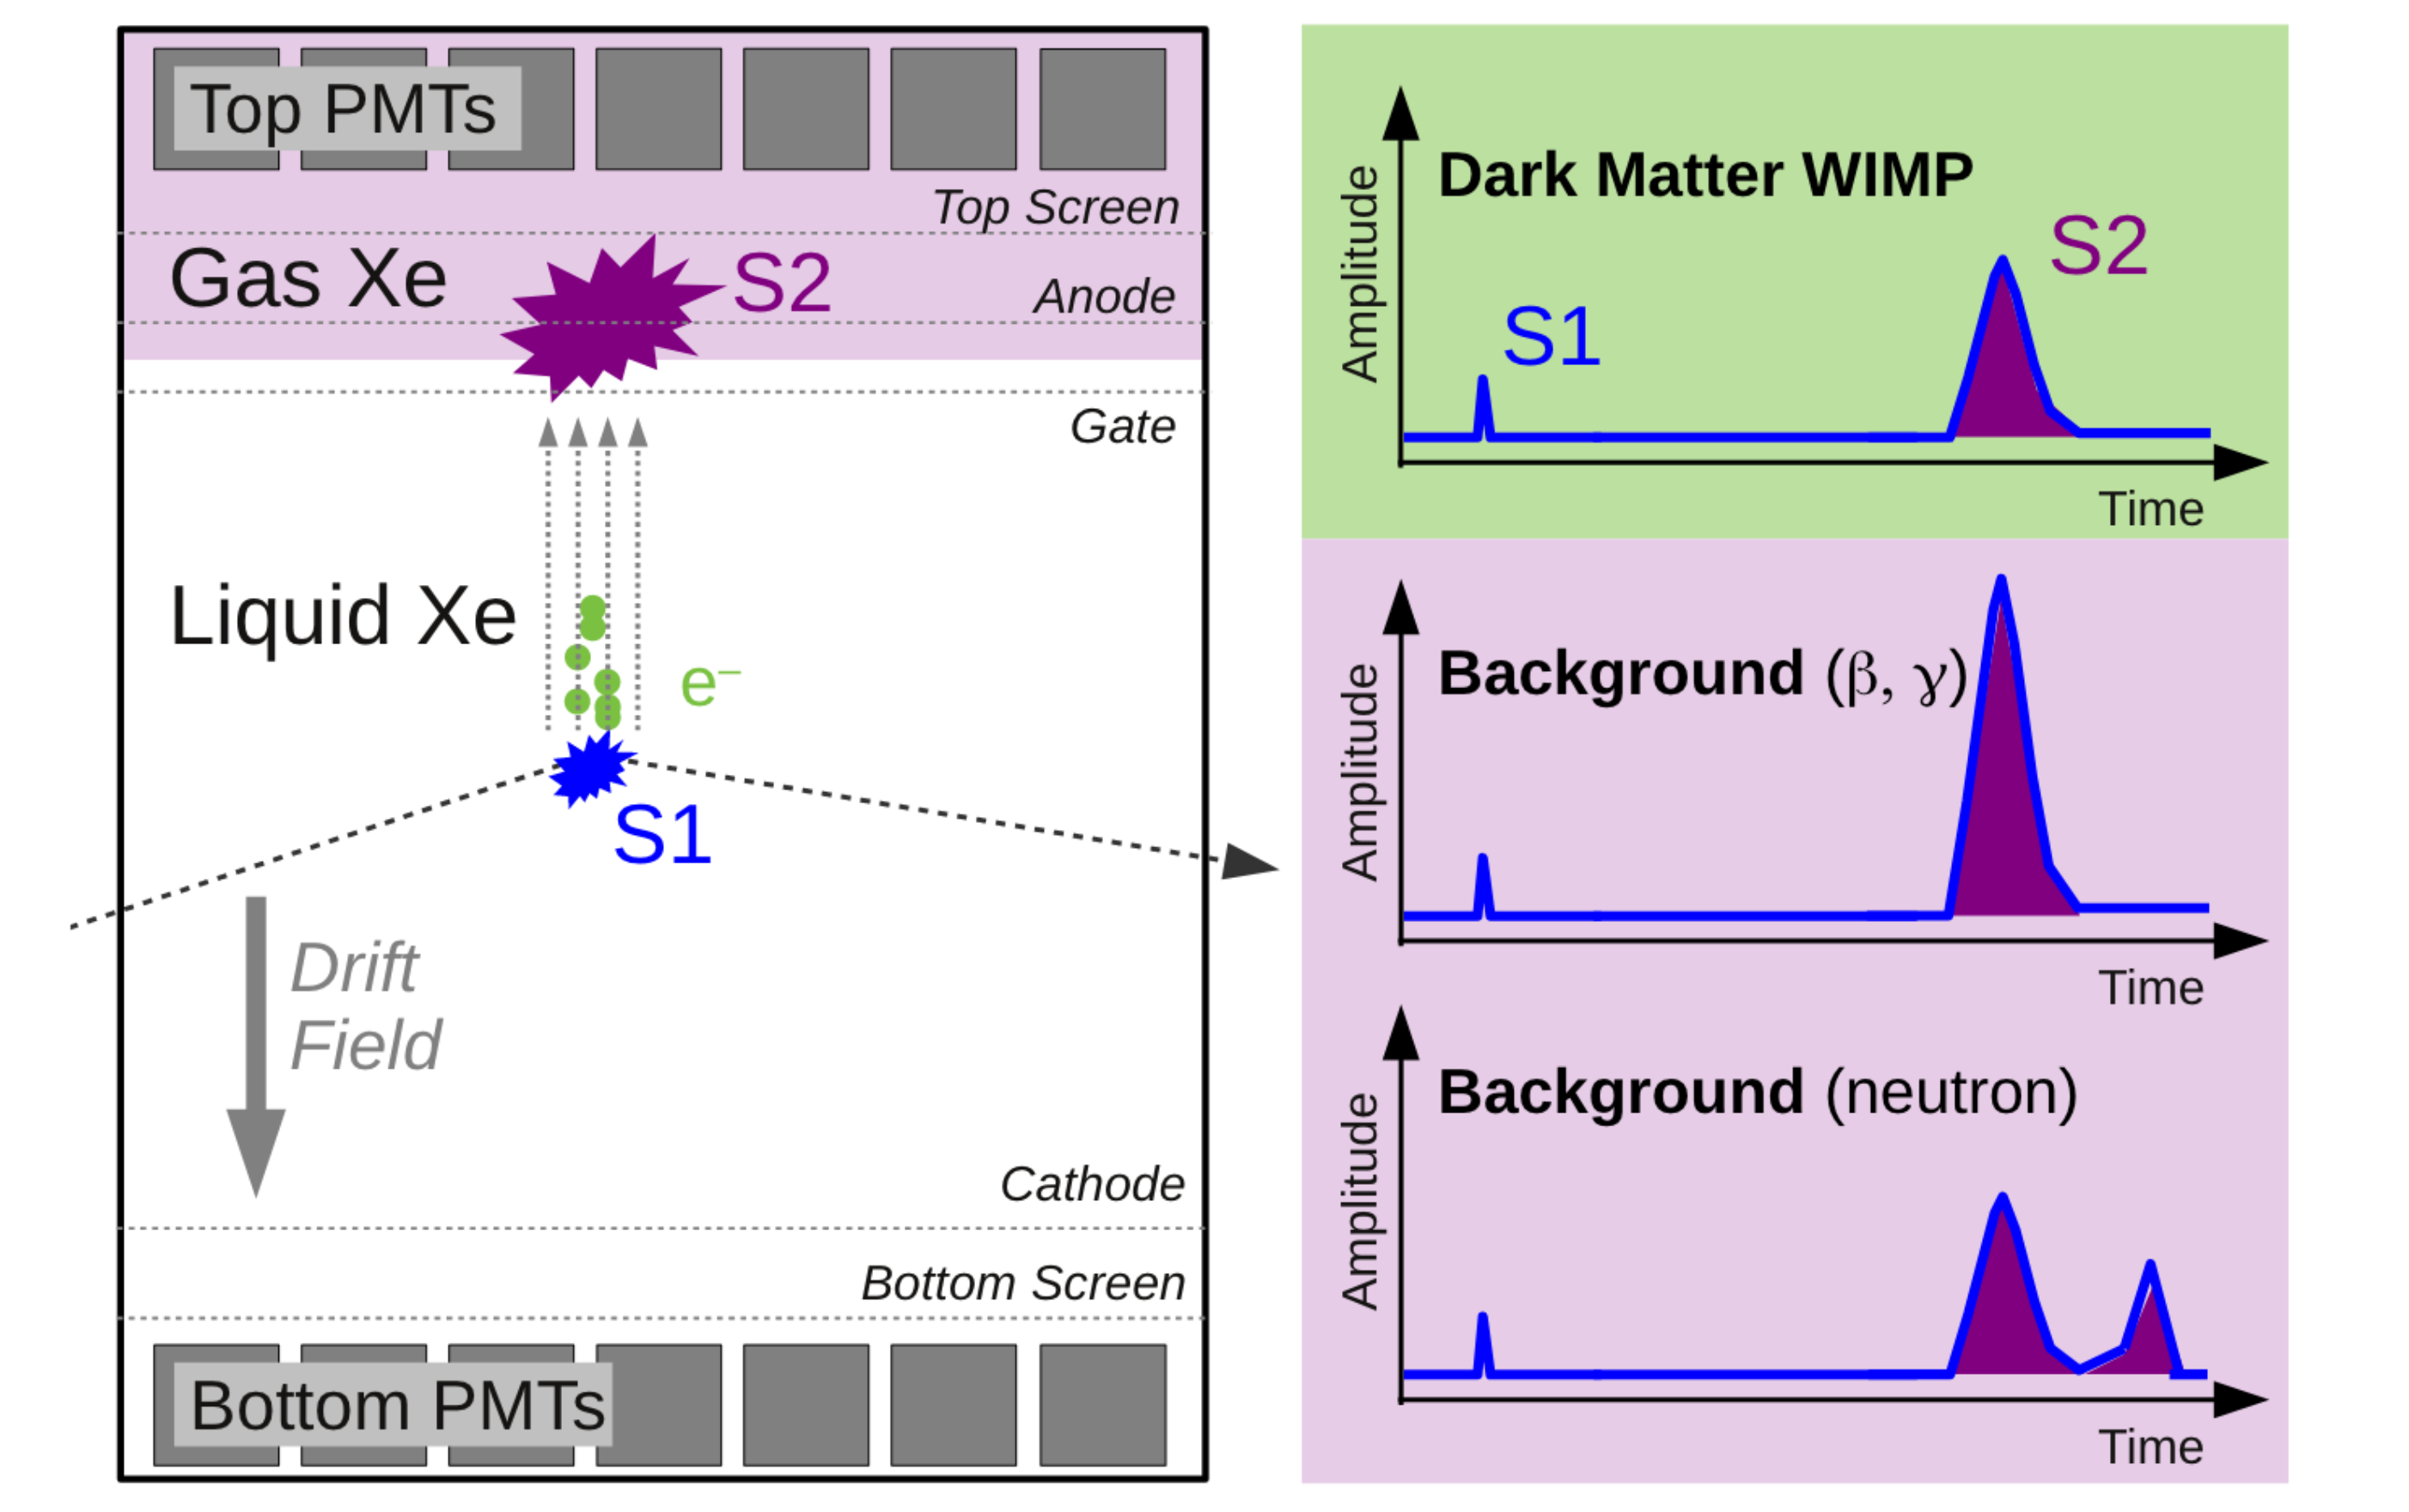
\includegraphics[width=0.4\linewidth]{figures/tpc_signals.png}
    \caption{LXeTPC工作原理示意图。TPC的上下端安装有两组光电倍增管(photomultiplier tube, PMT)阵列。
    当入射粒子,如WIMP或中微子,撞击$\mathrm{Xe}$原子核,闪烁光信号将被PMT阵列探测到。一组TPC电极会建立几段纵向电场。
    能量沉积最终转化为电离电子的动能,在阴极(Cathode)和门电极(Gate)之间纵向电场的作用下,
    电子向上漂移并在门电极和阳极(Anode)之间产生正比闪烁光,该闪烁光也会被PMT阵列探测到。\cite{xenon_collaboration_xenon1t_2017}。}
    \label{fig:tpc_principle}
\end{figure}

图\ref{fig:tpc_principle}简要呈现了LXeTPC的工作原理。圆柱形TPC分为上下气液两种相态,并安装5层电极。
从上至下,电极分别为上屏蔽(Top Screen),阳极,门电极,阴极和下屏蔽(Bottom Screen)。
上屏蔽和阳极在气氙中,其余三个电极浸泡在液氙中。
阴极和门电极之间建立均匀漂移电场,门电极和阳极之间有强电场,可以将液面下电子拉出。

入射的中子、中微子或WIMP携带能量与液氙中原子核碰撞,产生核反冲;
入射电子核$\gamma$光子与电子相互作用,相应地产生电子反冲(electronic recoil, ER)。

反冲能会激发或电离液氙,激发态的$\mathrm{Xe_2^*}$退激,
在灵敏体积中产生波长为178$\si{nm}$的闪烁光,称为$\mathrm{S1}$,闪烁光在液氙中传播,
经过一系列光学过程后被PMT阵列收集并在数据采集(data acquisition, DAQ)系统中被记录下来。
能量沉积也会产生电离信号,在漂移电场作用下,电子从阴极方向向门电极方向漂移,在门电极和阳极之间的电场中被拉出至液面,
并在气态氙中产生闪烁光,称为$\mathrm{S2}$。另外也有一部分能量沉积以热能形式耗散。
能量沉积产生光信号、电子信号和热能的比例由反冲的类型和能量决定,由此我们可以一定程度上区分电子反冲和核反冲信号。

探测器中事件的能量和位置重建对实现精确的信号探测及最终的物理目标是至关重要的。
事件发生的纵向位置 $z$可以通过$\mathrm{S1}$和$\mathrm{S2}$之间的时间差和电子漂移速度计算得出。
事件在TPC圆柱的上下表面投影位置可以通过顶部PMT阵列接收到的$\mathrm{S2}$图案通过位置重建算法得到。

\section{LXeTPC的响应模型}

液氙中有三种基本能量响应:热能耗散、氙原子激发和氙原子电离。LXeTPC一般不能探测热能。
液氙中的能量响应可以用NEST(the Noble Element Simulation Technique)模型描述\cite{szydagis_nest_2011,lenardo_global_2015}。
激发态的氙数目$N_{ex}$和被电离的电子-氙离子对个数$N_i$之和为可探测的量子(quanta)数$N_q$,
$N_q$可以用于重建反冲能$\epsilon$。在热能损失下,$N_q$服从二项分布:

\begin{align}
    \label{eq:N_q}
    N_q &\sim \mathrm{Binom}\left(\epsilon/W,L\right)
\end{align}

其中$L$为Lindhard因子,用于描述热能损失的比例;
$W$是能量沉积产生一个激发态氙或电子-氙离子所需平均能量,
实验测得$W=13.7\pm0.2\si{eV}$\cite{szydagis_nest_2011}。
在电子反冲过程中,因为电子质量远小于氙原子核质量,所以以热能损失的能量可以忽略不计;
在核反冲过程中,反冲氙原子以弹性散射方式向其周围氙原子传递动能,Lindhard因子$L$取值为$0.1\sim0.2$。
$L$对电场大小和反冲能量的依赖关系可以由NEST模型描述。

激发-电离比$\langle N_{ex}/N_i\rangle$反冲粒子对氙原子核的激发和电离截面有关。
对于电子反冲,这个值被认为是在0.06到0.20之间的常数。
对于核反冲,激发-电离比是沉积能量和灵敏体积内电场$F$的函数\cite{lenardo_global_2015}。
在$81\si{kV/cm}$电场下,$5-40\si{keV_{nr}}$的核反冲的激发-电离比在0.7到1.0之间。
$N_i$和$N_{ex}$的涨落可以用二项分布描述:

\begin{align}
    \label{eq:N_iex}
    N_i &\sim \mathrm{Binom}\left(N_q,\frac{1}{1+\langle N_{ex}/N_{i}\rangle}\right) \\
    N_{ex} &= N_q - N_i
\end{align}

电离电子有一定的几率$1-r$从电子-离子对中逃逸,$r$被称为重组比例(recombination ratio)。

\begin{align}
    \label{eq:N_er}
    N_e &\sim \mathrm{Binom}\left(N_i,1-r\right) \\
    N_\gamma &= N_i - N_e + N_{ex}
\end{align}

式\ref{eq:N_er}中,$N_\gamma$为激子推激以及电子-离子对重组放出的光子个数,$N_{e}$为逃逸的电子个数。
因为某些探测器效应,如电场不均匀性和某些内禀涨落\cite{lux_collaboration_tritium_2016},我们用正态分布来描述$r$:

\begin{align}
    \label{eq:r}
    r &\sim \mathrm{Gauss}\left(\langle r\rangle,\Delta r\right)
\end{align}

平均重组比例$\langle r\rangle$依赖于沉积能量大小和电场强弱,
其可以用Thomas-Imel(TI)箱模型描述\cite{thomas_recombination_1987}:

\begin{align}
    \label{eq:mr}
    \langle r\rangle &= 1 - \frac{\ln{\left(1+N_i\varsigma/4\right)}}{N_i\varsigma/4}
\end{align}

其中$\varsigma$是TI模型中的电场场强相关的参数。$\Delta r$描述了重组比例的涨落:

\begin{align}
    \label{eq:sr}
    \Delta r &= q_2\left(1-e^{-\epsilon/q_3}\right)
\end{align}

\section{地面运行的LXeTPC探测器设计}

\section{HPGe探测器的工作原理}
